\documentclass[10pt,a4paper]{article}
\usepackage[margin=2.2cm]{geometry}
\usepackage{fontspec}
\usepackage{kotex}
\setmainfont{Apple SD Gothic Neo}
\setsansfont{Apple SD Gothic Neo}
\usepackage{amsmath,amssymb}
\usepackage{graphicx}
\usepackage{booktabs}
\usepackage{caption}
\usepackage[dvipsnames]{xcolor}
\usepackage[colorlinks=true,linkcolor=MidnightBlue,citecolor=MidnightBlue,
            urlcolor=MidnightBlue]{hyperref}
\usepackage{titlesec}
\titleformat{\section}{\large\bfseries}{\thesection}{0.6em}{}
\titleformat{\subsection}{\normalsize\bfseries}{\thesubsection}{0.5em}{}
\captionsetup{font=small,labelfont=bf}
\setlength{\parskip}{0.35em}
\setlength{\parindent}{0pt}

\usepackage{mdframed}
\newmdenv[linewidth=0.4pt,linecolor=gray!60,backgroundcolor=gray!5,
          innertopmargin=6pt,innerbottommargin=6pt,skipabove=8pt,skipbelow=8pt]{claimbox}
\newcommand{\claim}[2]{\begin{claimbox}\textbf{주장.} #1\par\smallskip
  \textcolor{gray!70}{\textbf{반증 조건.} #2}\end{claimbox}}

\title{\bfseries 상설 챌린저\\[2pt]
\large 두 왕국의 국경이 장부가 됐다 --- 그리고 T$1$ 이 다시 열렸다}
\author{월드모델 실험실 · 노트 $804$}
\date{2026-08-07}
\begin{document}\maketitle

\section{한 줄}

논문 $167$ 이 결과로 고른 둘(아이돌·시장팝업)을 \textbf{못박힌 목록 · 새 씨앗
$4{\sim}7$} 로 다시 쟀다.

\begin{center}
\begin{tabular}{lrrrrr}
\toprule
& 챔피언 & TabPFN & 차(새 씨앗) & $803$ 대조 & $2\sigma$ \\
\midrule
아이돌 & $0.4515$ & $\mathbf{0.6315}$ & $\mathbf{+0.1800}$ & $+0.1698$ & $0.0367$ \\
시장팝업 & $0.1545$ & $\mathbf{0.2286}$ & $\mathbf{+0.0741}$ & $+0.0909$ & $0.0233$ \\
\bottomrule
\end{tabular}
\end{center}

\textbf{판정 (가) --- 둘 다 유지}($4.9$배 · $3.2$배 · 부호 뒤집힘 없음).
\emph{소외 도메인 보조 헤드}가 확정됐고, \texttt{lab/challenger.py} 에 \textbf{상설
챌린저 장부}를 세웠다(규약 $41$ · \texttt{--rerun} 포함). \textbf{T$1$(어떤 모델을
쓰나)이 이 세션에서 처음으로 다시 열렸다.}

\begin{figure}[t]\centering
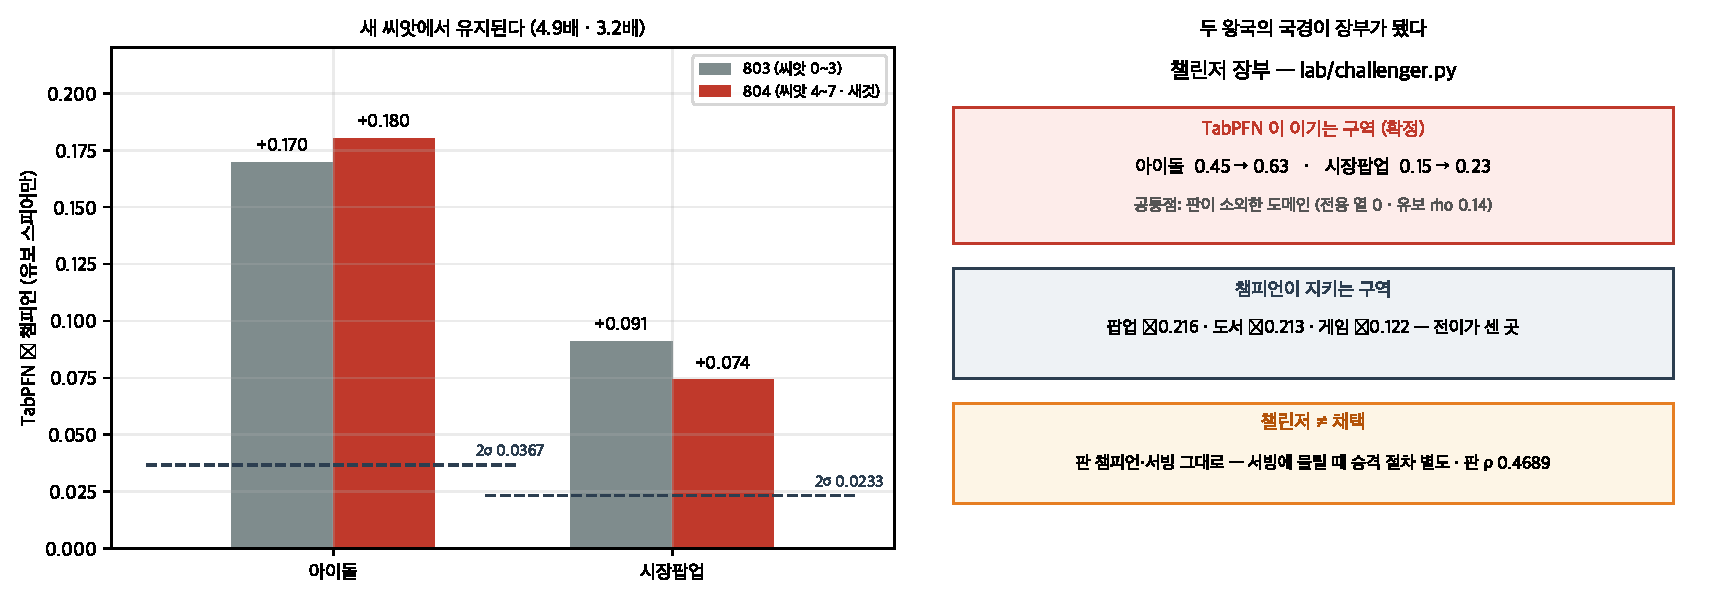
\includegraphics[width=0.92\textwidth]{figs/stand.pdf}
\caption{왼쪽: 두 씨앗 무리에서 같은 크기. 오른쪽: 장부의 세 칸 --- 이기는 구역 ·
지키는 구역 · 채택이 아니라는 못.}
\end{figure}

\section{챌린저는 채택이 아니다}

\claim{\textbf{판 챔피언과 서빙은 그대로다.} 장부는 \emph{``다른 모형이 어디서
얼마나 이기는가''}의 실측 기록이고, 서빙에 물릴 때 승격 절차를 따로 따진다.
이 구분이 없으면 챌린저의 국소 승리가 채택 규약(규약 $12$ 등)을 우회하는 뒷문이
된다 --- \textbf{아이돌 $+0.18$ 은 유혹적이지만 유보 $51$행짜리 도메인이고, 집 밖
검증이 없는 숫자다.}}
{서빙에 물리는 것을 막는 게 아니라 \textbf{절차를 요구하는 것}이다: 아이돌 축
배선(파일 $81$ 대 판 $173$ · 노트 $789$)을 고친 뒤에도 TabPFN 이 이기는지가 먼저다
--- \textbf{챔피언의 아이돌 성적이 배선 결함 때문이라면 고치는 쪽이 헤드를 다는
쪽보다 싸다.} T$1$ 미결로 적었다.}

\section{T$1$ 의 답이 모양을 갖췄다}

T$1$ 의 물음(\emph{어떤 모델을 쓰나})에 이 세션이 준 답: \textbf{단일 모형이
아니라 구역별 분업이다.} 합동 적합(전이)은 뿌리·수혜 도메인을 지키고, SCM
사전(단독 TabPFN)은 판이 소외한 도메인에서 이기고, 드리프트 보정(노트 $802$)은
절대값 층을 연다. \textbf{다음 측정}: 동결 임베딩 병기(사용자 로드맵 A$1$ ·
같은 챌린저 장부 · 리더보드 불신 조항).

\end{document}
